\scanpage{47}
\mspage{\handwritten{15}}
un $\handwritten{\mathcal{O}}_S$-Module plat $\handwritten{\unsure{\mathcal{A}|a}}$ , et $\handwritten{\mathcal{E}}$ un $\handwritten{\mathcal{O}}_S$-Module quasi-cohérent. On suppose soit que $G$ est affine\inserted{\handwritten{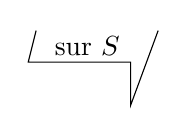
\begin{tikzpicture}[x=1cm,y=1cm,baseline=(n.base)]\node (n) at (0,0) {sur $S$};\draw (-.65,.2)--(-.75,-.2)--(.55,-.2)--(.55,-.75)--(.9,.2);\end{tikzpicture}}}, soit que \deleted{\unsure{G e}}t $\handwritten{\mathcal{E}}$ \deleted{son}\handwritten{soi}t plat\deleted{s} sur $S$. Soit $\handwritten{\rho:\mathcal{E}\to\mathcal{A}\otimes\mathcal{E}}$ un homomorphisme définissant une opé-\linebreak ration de $G$ sur $\handwritten{\mathcal{E}}$. Soit $\handwritten{\mathcal{E}}_{\unsure{o|0}}$ un sous-$\handwritten{\mathcal{O}}_S$-Module quasi-cohérent de $\handwritten{\mathcal{E}}$ tel que l'homomorphisme $\handwritten{\mathcal{E}}_{\unsure{o|0}}\handwritten{\longrightarrow\mathcal{A}\otimes\mathcal{E}}$ déduit de $\handwritten{\rho}$ se factorise à travers l'homomorphisme canonique \handwritten{(}injectif\inserted{\handwritten{, grâce au 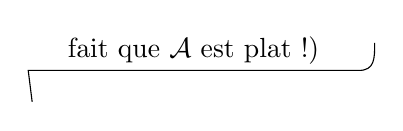
\begin{tikzpicture}[x=1cm,y=1cm,baseline=(n.base)]\node (n) at (0,0) {fait que $\mathcal{A}$ est plat !)};\draw (-2.05,-.65)--(-2.1,-.25)--(2.1,-.25) .. controls (2.3,-.25) and (2.3,-.1) .. (2.3,.1);\end{tikzpicture}}} $\handwritten{\mathcal{A}\otimes\mathcal{E}_{\unsure{o|0}}\longrightarrow\mathcal{A}\otimes\mathcal{E}}$ au moyen de l'homomorphisme $\handwritten{\rho_{\unsure{o|0}}:\mathcal{E}_{\unsure{o|0}}\longrightarrow\mathcal{A}\otimes\mathcal{E}_{\unsure{o|0}}}$. Alors $\handwritten{\rho_{\unsure{o|0}}}$ définit une opération de $G$ sur $\handwritten{\mathcal{E}_{\unsure{o|0}}}$\handwritten{(},\handwritten{(} qu'on appellera \uline{opération induite} sur $\handwritten{\mathcal{E}}_{\unsure{o|0}}$ par $\handwritten{\rho}$, et on dira que $\handwritten{\mathcal{E}}_{\unsure{o|0}}$ est \uline{stable} sous $\handwritten{\rho)}$.

Cela résulte immédiatement des définitions et de (11.\handwritten{6}). On remarquera cependant qu'en général l'application canonique $\handwritten{\mathbb{W}}(\handwritten{\mathcal{E}}_{\unsure{o|0}})\handwritten{\longrightarrow\mathbb{W}}(\handwritten{\mathcal{E}})$ n'est pas injective.

\uline{Lemme 11.8.}- \uline{Soient $G$ un $S$-groupe quasi-séparé et quasi-compact sur $S$ tel que $\handwritten{\mathcal{A}}(G)$ soit un $\handwritten{\mathcal{O}}_{\unsure{\mathbb{S}|S}}$-Module \deleted{\unsure{plat} $\handwritten{\mathcal{A}}$,} libre $\handwritten{\mathcal{A}}$ de base $(\handwritten{\varphi}_i)$, $\handwritten{\mathcal{E}}$ un $\handwritten{\mathcal{O}}_S$-Module quasi-cohérent. On suppose soit que $G$ est affine\inserted{\handwritten{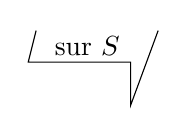
\begin{tikzpicture}[x=1cm,y=1cm,baseline=(n.base)]\node (n) at (0,0) {sur $S$};\draw (-.65,.2)--(-.75,-.2)--(.55,-.2)--(.55,-.75)--(.9,.2);\end{tikzpicture}}}, soit que $G$ et $\handwritten{\mathcal{E}}$ sont plats sur $S$. Soit $\handwritten{\rho:\mathcal{E}\to\mathcal{A}\otimes\mathcal{E}}$ un homomorphisme définis-\linebreak sant une opération de $G$ sur $\handwritten{\mathcal{E}}$, et soit $x\handwritten{\in\Gamma}(S,\handwritten{\mathcal{E}})$. Posons $\handwritten{\rho}(x)=\handwritten{\sum\varphi}_i\handwritten{\otimes x}_i$, où les $x_i\handwritten{\in\Gamma}(S,\handwritten{\mathcal{E}})$ sont bien déterminés par cette relation). Alors le sous-module\inserted{\handwritten{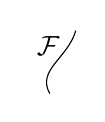
\begin{tikzpicture}[x=1cm,y=1cm,baseline=(n.base)]\node (n) at (0,0) {$\mathcal{F}$};\draw (.35,.2) .. controls (.25,-.15) and (-.15,-.3) .. (.02,-.6);\end{tikzpicture}}} de $\handwritten{\mathcal{E}}$ engendré par les $x_i$ est stable sous $\handwritten{\rho}$,\deleted{et contient $x$.}\inserted{quasi-cohérent} et de type fini sur $\handwritten{\mathcal{O}}_S$, et $x\handwritten{\in\Gamma}(S,\handwritten{\mathcal{F}})$.}
\figure{\handwritten{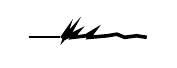
\begin{tikzpicture}[x=1cm,y=1cm]\draw[line width=.7pt] (0,0) -- (.4,0);\draw[line width=1.3pt] (.42,-.01) -- (.49,.09) -- (.46,0) -- (.55,.1) -- (.5,.01) -- (.62,.07) -- (.56,0) -- (.73,.02) -- (.83,.08) -- (.77,0) -- (1,.02) -- (1.12,.04) -- (1.22,0) -- (1.37,.02) -- (1.5,0);\end{tikzpicture}}}

\deleted{Soit $\handwritten{\mathcal{F}}$ le sous-module de $\handwritten{\mathcal{E}}$ engendré par les $x_i$\unsure{,|.}} \handwritten{I}l est clair que $\handwritten{\mathcal{F}}$ est quasi-cohérent et de type fini. L'axiome (CM1) montre que $\handwritten{\sum\Delta}(\handwritten{\varphi}_i)\handwritten{\otimes}x_i=\handwritten{\sum\varphi}_i\handwritten{\otimes\rho}(x_i)$ ; d'autre part, $\handwritten{\Delta(\varphi}_i\handwritten{)=\sum\varphi}_j\handwritten{\otimes}a_{ij}$ , d'où $\handwritten{\sum\varphi}_j\handwritten{\otimes}a_{ij}\handwritten{\otimes}x_i=\handwritten{\sum\varphi}_i\handwritten{\otimes\rho}(x_i)$, d'où, puisque les $\handwritten{\varphi}_i$ forment une base de $\handwritten{\mathcal{A}}$, $\handwritten{\rho}(x_i)=\handwritten{\sum}a_{ji}\handwritten{\otimes}x_{\handwritten{i}}$, où $a_{ji}\handwritten{\in\Gamma}(S,\handwritten{\mathcal{A}})$, ce qui montre que $\handwritten{\rho(\mathcal{F})\subset\mathcal{A}\otimes\mathcal{F}}$, donc $\handwritten{\mathcal{F}}$ est stable sous $\handwritten{\rho}$. Enfin l'axiome (CM2) montre que $x=\handwritten{\sum_i\eta}(\handwritten{\varphi}_i)x_i\handwritten{\in\Gamma}(S,\handwritten{\mathcal{F}})$.

\uline{Proposition 11.9.- Soit $G$ un $S$-groupe quasi-compact quasi-séparé sur $S$ tel que $\handwritten{\mathcal{A}}=\handwritten{\mathcal{A}}(G)$ de-\linebreak vienne localement libre après extension fidèlement plate quasi-compacte de la base $S$ (ce qui} est le cas\inserted{\handwritten{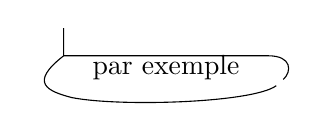
\begin{tikzpicture}[x=1cm,y=1cm,baseline=(n.base)]\node (n) at (0,0) {par exemple};\draw (-1.3,.5)--(-1.3,.15) .. controls (-1.75,-.2) and (-1.5,-.3) .. (-1.2,-.38) .. controls (-.6,-.5) and (1.1,-.45) .. (1.4,-.23);\draw (-1.3,.15)--(1.3,.15) .. controls (1.6,.15) and (1.6,-.05) .. (1.49,-.15);\end{tikzpicture}}} lorsque $G$ est un groupe réductif, comme nous\deleted{\unsure{l}} le verrons dans \deleted{l'exposé} \handwritten{$\overline{\underline{\mathrm{XXV}}}$}), \uline{et} \uline{soit $\handwritten{\mathcal{E}}$ un $\handwritten{\mathcal{O}}_S$-\deleted{module}\handwritten{Module} quasi-cohérent . On suppose soit que $G$ est affine\inserted{\handwritten{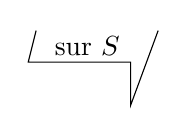
\begin{tikzpicture}[x=1cm,y=1cm,baseline=(n.base)]\node (n) at (0,0) {sur $S$};\draw (-.65,.2)--(-.75,-.2)--(.55,-.2)--(.55,-.75)--(.9,.2);\end{tikzpicture}}}, soit que $G$ et $\handwritten{\mathcal{E}}$ sont plats sur $S$. Soit $\handwritten{\rho:\mathcal{E}\longrightarrow\mathcal{A}\otimes\mathcal{E}}$ un homomorphisme définissant une opération de $G$ sur $\handwritten{\mathcal{E}}$.}
% archive sheet number: 46
